\chapter{Resultados para el mapeo de asignación}

\section{Parte analítica}


\subsection{SWAP}
\subsubsection{Estado fino compatible arbitrario}
Sea $\rho\in\mcL(\mcH_{2})$ un estado grueso sobre z definido como en (\ref{eq:rhoz}) y $\varrho$ un estado fino compatible con parametrización de Bloch $\vec{\gamma}$. Sabemos que la acción del coarse graining sobre $\varrho$ es
\begin{equation}\label{eq:CGSWAPprei}
\CG{\varrho}=\frac{1}{2}\qty(\Id+\sum_{k=1}^{3}(p\gamma_{k,0}+(1-p)\gamma_{0,k})\sigma_{k}).
\end{equation}
Este estado, claro, debe estar alineado con el eje $z$, así que se cumple que $p\gamma_{k,0}+(1-p)\gamma_{0,k}=0$ para $k=1,2$. De esta forma, el estado queda como
\begin{equation}\label{eq:CGSWAPi}
\CG{\varrho}=\frac{1}{2}\qty(\Id+(p\gamma_{3,0}+(1-p)\gamma_{0,3})\sigma_{z}).
\end{equation}
Luego, si se aplica el SWAP, el estado grueso efectivo es
\begin{equation}\label{eq:CGSWAPfi}
\CG{S\varrho S}=\frac{1}{2}\qty(\Id+\sum_{k=1}^{3}(p\gamma_{0,k}+(1-p)\gamma_{k,0})\sigma_{k}).
\end{equation}
Para que las ecuaciones (\ref{eq:CGSWAPi}) y (\ref{eq:CGSWAPfi}) correspondan al mismo estado (esto es, que la dinámica efectiva sea la identidad), primero debe de cumplirse que $p\gamma_{0,k}+(1-p)\gamma_{k,0}=0$ para $k=1,2$. Si se combinan ambas condiciones sobre estas componentes se obtiene
\begin{align*}
(2p-1)(\gamma_{k,0}-\gamma_{0,k})&=0,\\
\gamma_{k,0}+\gamma_{0,k}&=0.
\end{align*}
Esto asegura que el estado descrito por (\ref{eq:CGSWAPfi}) esté sobre el eje z, pero para que la coordenada en dicho eje no cambie tras el SWAP subyacente debe cumplirse que 
\begin{equation*}
(2p-1)(\gamma_{3,0}-\gamma_{0,3})=0,
\end{equation*}
De esta forma, puede verse que un estado $\psi$ que cumpla que $\gamma_{k,0}=\gamma_{0,k}=0$ para $k=1,2$ y que $\gamma_{3,0}=\gamma_{0,3}$ no se ve afectado por el SWAP de forma efectiva. Esta invarianza es completamente dependiente del estado fino inicial (o del estado grueso inicial), y las condiciones sobre las componentes se cumplen \notaAd{solo si, estoy seguro de que si se revisan las constantes de estructura sí sale el solo si} si $\rho_{z}$ es puro, y por consiguiente $\varrho=\rho_{z}\otimes\rho_{z}$.

Además, la dinámica efectiva es la identidad siempre que $p=0.5$. Para dicho valor de $p$ se satisfacen todas las condiciones.

\subsubsection{Mapeo de asignación}

Sea $\{\varrho^{j}\}_{j=1}^{N}$ el conjunto usado en el mapeo de asignación, y $\{\vec{\gamma}^{j}\}_{j=1}^{N}$ el conjunto de sus parametrizaciones de Bloch. En tal caso los estados efectivos inicial y final son:
\begin{align}
\rho&=\frac{\sigma_{z}}{N}\sum_{j}(p\gamma_{3,0}^{j}+(1-p)\gamma_{0,3}^{j}),\\
\rho'&=\frac{\sigma_{z}}{N}\sum_{j}(p\gamma_{0,3}^{j}+(1-p)\gamma_{3,0}^{j}).
\end{align}
La dinámica efectiva vuelve a ser la identidad si $p=0.5$ o si $\rho_{z}$ es puro


\newpage


\section{Parte numérica}
\subsection{Cascarón de estados mixtos}
Se generan estados puros $\begin{pmatrix}
a\\
b\\ \end{pmatrix}$ de manera uniforme. Estos son puntos en el cascarón unitario. Todos estos puntos se deplazan radialmente hacia adentro mediante un factor:
\begin{equation}
\vec{\alpha}=r\vec{\alpha_{0}}
\end{equation}
El resultado es un conjunto de estados mixtos $\{\rho_{i}\}_{i=1}^{N}$ cuyos vectores de Bloch se encuentran en el cascarón de radio $r$.

\subsubsection{Mapeo de asignación para el cascarón}


A cada $\rho_{i}$ hay que hallarle su estado fino asignado. Lo que se hace es generar un conjunto $\{\psi_{i}\}_{i=1}^{N}$ de estados finos para un estado grueso en $z$, $\rho_{z}$, tal que su coordenada en $z$ es justamente el radio del cascarón.

Como existe una unitaria $U_{i}$ entre $\rho_{z}$ y cada estado de $\{\rho_{i}\}_{i=1}^{N}$. Entonces podemos aplicar estas unitarias para hallar todos los $\mcA[\rho_{i}]$.

\subsection{Resultados}

Dos experimentos. En el primero se utiliza una probabilidad de swap $p=0.5$ (cascarón de radio $r=0.3$). El conjunto no cambia. En el segundo se utiliza una probabilidad de swap $p=0.3$ (cascarón de radio $r=0.8$).

Se grafican dichos cascarones en azul. Se aplica un SWAP a todos los $\mcA[\rho_{i}]$, y se saca el coarse graining. El resultado se grafica en amarillo.

\begin{figure}[h]
\centering
\begin{subfigure}{0.4\textwidth}
  \centering
  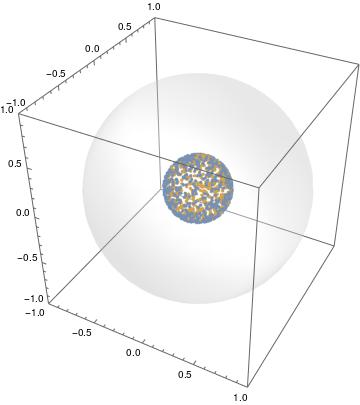
\includegraphics[width=0.8\linewidth]{assmap/figures/effectiveswap_p=0.5_z=0.3.jpeg}
  \caption{$p=0.5$, $r=0.3$, el conjunto no cambia después del swap subyacente}
  \label{fig:paralelogram}
\end{subfigure}
\begin{subfigure}{0.4\textwidth}
  \centering
  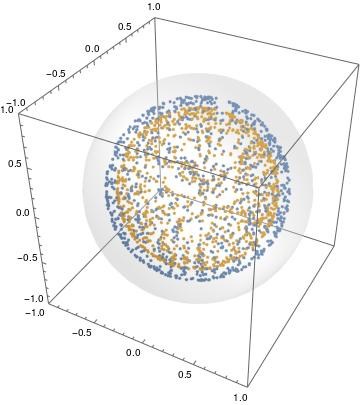
\includegraphics[width=0.8\linewidth]{assmap/figures/effectiveswap_p=0.3_z=0.8.jpeg}
  \caption{$p=0.5$, $r=0.3$, el conjunto se contrae  después del swap subyacente}
  \label{fig:paralelogram}
\end{subfigure}
\label{fig:cooldensities}
\end{figure}